\chapter[Estado da Arte]{Estado da Arte}
Esta sessão traz todo referencial teórico necessário para desenvolver o projeto
de aplicação do \textit{Octalysis}, contemplando tópicos explicativos sobre os subsídios
necessários para suporte na construção deste. Este capítulo contempla três sessões.
A sessão \ref{sec:gamifição} trata sobre o contexto de gamificação atual, qual a
sua funcionalidade e qual a sua aplicação na sociedade, bem como a apresentação
de um \textit{Framework} consolidado para o seu desenvolvimento. A sessão \ref{sec:redessociais}
trata sobre Redes Sociais com a proposta que vai de encontro com a linha da RSA.
Por fim, na sessão \ref{sec:processo_de_desenvolvimento_de_software},
éapresentado uma visão geral sobre processos de
Desenvolvimento de \textit{Software}, bem como a Metodologia que é aplicada e utilizada
para a conclusão do projeto estipulado.

\section{Gamifição}
\label{sec:gamifição}
A gamifição, apesar deste nome, não remete que uma dada ferramenta é um jogo,
como dito por \cite{popularitygamification}, este processo é o emprego de
várias funcionalidades e características presentes em \textit{Games} em uma determinada
plataforma. Este utiliza como exemplo a palavra \textit{game-fy-ing}, que nos sugere
exatamente o fato de aplicar estas características de \textit{Game} dentro de algo.

A aplicação e a diferença entre \textit{game} e gamifição fica evidenciada
no estudo de \cite{deterding2011gamification}, onde estes afirmam que a gamifição contém  apenas
um uso dos elementos das características de \textit{design} de \textit{games}, tudo isso,
aplicado em contextos que não são \textit{games}. O que é totalmente diferente
de um \textit{design} produzido unicamente para jogos.

A primeira vez que se tem registro do uso do termo gamifição foi em 2002,
por \cite{pelling}, mas ainda assim este termo não foi aplicado e comumente
utilizado. Apenas no final de 2010, como dito por \cite{deterding2011gamification}, que
este termo foi adotado como uma maneira não de transformar algo em um \textit{game},
mas de aplicar e aproveitar todas as características positivas deste em uma dada
plataforma.

Todo o processo de gamifição aplicado a qualquer plataforma se basea em
quatro blocos, que podem ser características advindas dos \textit{games}. Podem ser
aplicados os seguintes pontos, com alguns a mais ou a menos, a depender
do perfil do profissional que está desenhando a gamifição, segundo \cite{mcgonigal2011reality}.
Os quatro pontos são os seguintes:

\begin{itemize}
    \item Objetivo;
    \item Regras;
    \item Sistema de \textit{Feedback};
    \item Participação voluntária.
\end{itemize}

O pensamento de \cite{deterding2011gamification}  sobre a divisão clara entre jogos sérios
de jogos de diversão e a gamificação é colocado em um diagrama, onde este
apresenta os limites de cada parte. Este pensamento, desenhado em um diagrama,
está apresentado na Figura \ref{fig:gamificacaodetalhada}. Este modo de pensar é interessante, pois
é similar à composição de jogos, composta por \cite{mcgonigal2011reality}, onde este
propõe uma sequência de regras, participações voluntárias, sistema de
\textit{feedbacks} e metas, que são todos feitos e elaborados para um contexto que
não é de aplicação de um jogo, chamados de não jogo. A figura \ref{fig:gamificacaodetalhada}
também se enquadra no mesmo pensamento e perspectiva de \cite{mcgonigal2011reality}.

\begin{figure}[h]
    \centering
    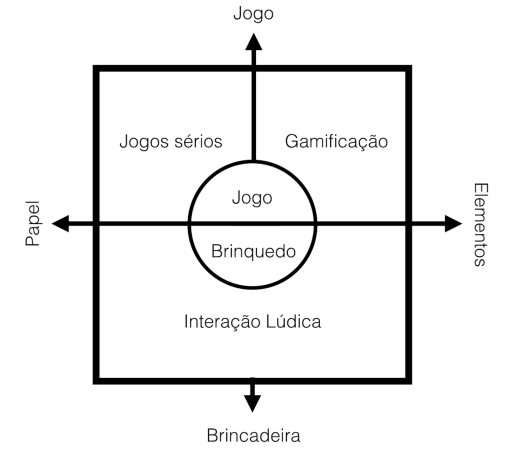
\includegraphics[width=400px, scale=1]{figuras/gamificacaodetalhada}
    \caption{Definição detalhada de gamificação. }
    \label{fig:gamificacaodetalhada}
\end{figure}


Sobre motivações e engajamento, \cite{chou2015actionable}  defende que as motivações
do usuário vem bem antes das execuções das mecânicas dos jogos. Este defende
que as mecânicas dos jogos não são os verdadeiros motivos de um jogo ser
engajado, mas sim, a motivação do usuário em usá-lo, fazendo com que seja
necessário pensar, avaliar e projetar o que o usuário deseja sentir. \cite{chou2015actionable} define que a gamificação é uma forma diferente de derivar o engajamento
e a motivação  que comumente é encontrada nos jogos, fazendo essa afirmação
mesmo acreditando que a discussão seja válida para a comunidade.

Assim, dessa forma, temos a definição de \cite{zichermann2011gamification} sobre qual é o conceito de
gamifição, afirmando que este é um processo de pensamento da aplicação assim
como jogador e fazendo a utilização
de mecanismos de \textit{game} que servem para enganjar e motivar os usuários a utilizarem
determinada funcionalidade e resolver problemas.

Autor, em seu estudo, defende o quão importante a gamifição é na definição
de alguma plataforma. Ele utiliza a pergunta: "\textit{Why Gamify?}". Assim, este defende
que a gamifição é uma ferramenta poderosa, que consegue capturar com habilidade
a atenção de pessoas para alguma atividade alvo definida.

Autor ainda defende  o poder da gamifição com alguns exemplos práticos,
como a utilização por 18 milhões de pessoas em todo o mundo do jogo Nike+.
Além da interessante utilização modificada dos jogadores de
\textit{Piano Stairs} que jogam em \textit{Odenplan}, onde sessenta e seis porcento destes
escolheram a opção de escada e não a opção de elevador.

\subsection{Modelos de Bartle}
\label{sub:modeloBartle}
O estudo proposto por \cite{bartle1996hearts} aponta que normalmente, os jogadores
tem perfis definidos. Que, por mais que ele pense para várias situações
, é normal que o indivíduo tenha um ponto e uma característica que prevaleça
perante as demais. Essas características estão embasadas nos objetivos
que o usuário  busca alcançar com o uso da plataforma presente.
Alguns desejos de caráter conquistador, outros, explorador, que gostam
de desvendar, já outrem, estão interessados apenas em interação
social. Os perfis definidos são os seguintes:


\begin{itemize}
    \item Conquistador: é o perfil de usuário que seu único objetivo é acumular o
        que há de riqueza dentro do jogo, seja pontos, moedas, ações ou afins.
        Tudo o que ele faz é com o objetivo de conquistar mais bens. Caso ele explore
        o jogo, a procura de novos caminhos, seu objetivo é conquistar pontos com
        isso, se ele desafia os usuários, seu objetivo é conquistar bens. Se ele
        tem atitudes sociais, todas elas são para conquistar mais pontos e mais riquezas;
    \item Exploradores: são aqueles que fazem e movem tudo por descobrir aquilo
        que está obscuro no jogo, que tem vontade de ver o que há de novo e seus desafios
        são cunhados na capacidade de conhecer e desvendar novos eventos. A motivação
        deste é unicamente fazer atividades com o objetivo de conseguir descobrir mais.
        Caso este tenha que ter pontos para descobrir algo, então, o fará. Assim
        como socializar ou combater alguém;
    \item Assassinos: são os usuários com perfil que tem desejo por demostrar a sua
        supremacia de poder diante dos outros usuários, que gostam de aplicar
        e mostrar a sua força, com o perfil de assassino. Sua satisfação
        é diretamente ligada ao poder que este impõe ao adversário, mostrando
        o quão este tem mais autoridade. Conquistar pontos, para o assassino, é uma forma
        de se tornar mais poderoso, explorar é uma forma de adquirir mais habilidades,
        socializar é uma forma de conhecer novas táticas de batalha com os demais
        usuários;
        % eugenio.semprebone
    \item Socializadores: seu foco e motivação é conhecer e criar relacionamento
        com outras pessoas. Todo o ambiente do jogo é apenas um meio para que
        os laços sejam criados. O jogo em si pouco importa, mas sim os relacionamentos
        que podem ser criados dentro do ambiente. Para o socializador, explorar pode
        ser necessário para entender os pontos nos quais o resto do mundo está tratando;
        Acumular pontos é necessário para conseguir ter acesso a níveis desconhecidos
        e que impede que as relações sejam feitas. Já utilizar práticas assassinas são
        executadas em último caso, apenas se for necessário para continuar sua trajetória
        durante o \textit{game}.
\end{itemize}

Para a definição destes usuários, \cite{bartle1996hearts} desenvolveu um gráfico que demonstra o
interesse dos jogadores segundo seu perfil. Este gráfico tem duas variáveis dispostas
em dois eixos. O eixo Y representa o tipo de ação dos jogadores, já o eixo X define
em que tipo de perfil as ações são tomadas.

No eixo Y, tem-se a diferença entre jogadores
que tomam ações atuando diretamente no jogo ou interagindo. Já no eixo X, temos as ações,
que são aplicadas de um lado nos jogadores e por outro lado, são aplicadas no mundo como
um todo. Estas diferenças podem ser observadas na Figura \ref{fig:perfiljogadores} a seguir:

\begin{figure}[h]
    \centering
    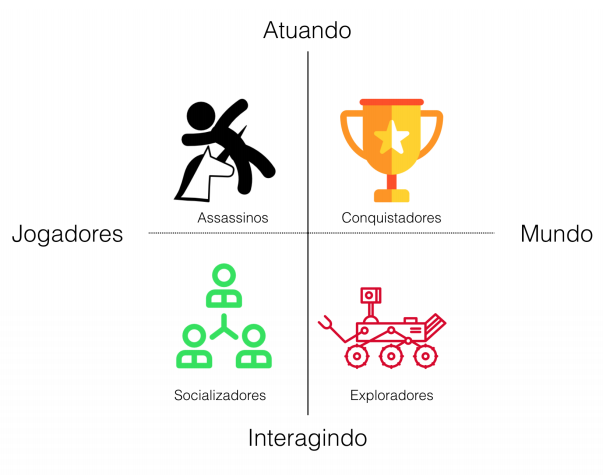
\includegraphics[width=400px, scale=1]{figuras/perfiljogadores}
    \caption{Perfis de jogadores.}
    \label{fig:perfiljogadores}
\end{figure}


\subsection{Modelos centrados no ser humano}
\label{sub:modelosnoserhumano}
Existem no mercado vários \textit{Frameworks} e projetos que tem como finalidade o ser
humano que está por trás do que está sendo gamificado. Além disso, há
vários processos de gamificação que tem como base esta filosofia. 
\cite{kumar2013gamification}
cunhou este termo, também sendo utilizado por \cite{chou2015actionable} em seu projeto.
Estes dois projetos demonstrados a seguir nesta sessão. O primeiro
deles é o modelo de Kumar, sendo o segundo o \textit{Framework} Octalysis, de Yu-kai Chou.

\subsubsection{Modelo de Kumar}
\label{sub:modelodekumar}
O modelo de Kumar sugere que antes de fazer qualquer projeto e aplicar qualquer gamificação,
é necessário entender o tipo de usuário que está em jogo, qual a categoria de usuário
que está sendo discutida. Dessa forma, é possível aplicar traços de gamificação
que condizem com a perspectiva do usuário, e assim, fazer com que este aproveite
mais das características que serão cunhadas. Após a elaboração do contexto do
usuário, se faz necessário definir e entender a missão e identificar qual o negócio
desejado para o ponto ressaltado.

Logo após o entendimento por completo do contexto e das razões de negócio do
produto, é possível aplicar as mecânicas de jogo no contexto que é totalmente
não jogo. Assim, é possível obter, de acordo com o que o usuário necessita, as
dinâmicas de jogo corretas. A figura \ref{fig:Kumar} indica e mostra a propriedade de
como se organiza o diagrama. É possível observar que a motivação, a missão e a
mecânica estão todas em volta, trabalhando a favor do jogador, sendo que estas
três devem ser modeladas para este usuário.

\begin{figure}[h]
    \centering
    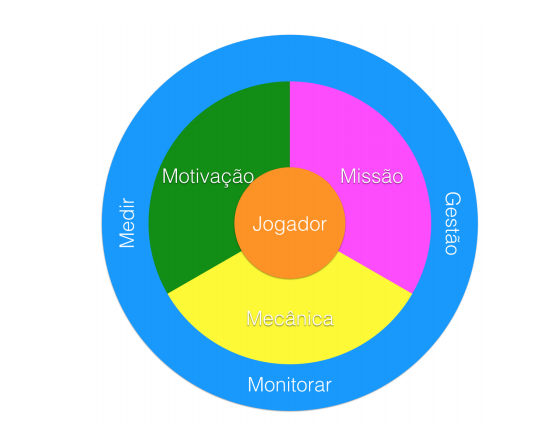
\includegraphics[width=400px, scale=1]{figuras/kumar}
    \caption{ \textit{Design} centrado no ser humano.}
    \label{fig:Kumar}
\end{figure}

Além da missão, motivação e mecânica é necessário que haja todo um gerenciamento
destes três pontos, para ajustá-los de acordo com os \textit{feedbacks} do usuário. Dessa
maneira, a cada interação, o \textit{Framework} deve passar por um ponto de monitoramento,
medição e gerenciamento dos variantes. Para que assim, seja possível monitorar e
avaliar o quão é necessário modificar as estratégias de negócio.

\subsubsection{Modelo de Yu-kai Chou}
\label{sub:modelodeyu-kaichou}
Este é um modelo que o principal foco é o personagem humano, que está do lado
de fora do jogo. \cite{chou2015actionable} acredita que o usuário vem antes de qualquer evento
dentro de uma gamificação. A sua intenção, elaborando um novo \textit{design} de projeto
de gamificação, é quebrar o paradigma de que esta deve ter um foco funcional,
apenas para obter resultados rápidos. Este acredita que a função da gamificação
deve vir para engajar e motivar o ser humano, e para isso, é nessário entender o
que está por trás de tudo isso, ou seja, as pessoas que estão para ter o
potencial de engajamento aumentado.

Chou desenvolveu um \textit{Framework} que este intitulou de Octalysis, no qual atribuiu
este nome devido as oito faces de motivações básicas do usuário definido por ele.
Este esquema é representado pelas motivações básicas, uma em cada face do Octalysis,
como representado na figura \ref{fig:octalysisex}.

\begin{figure}[h]
    \centering
    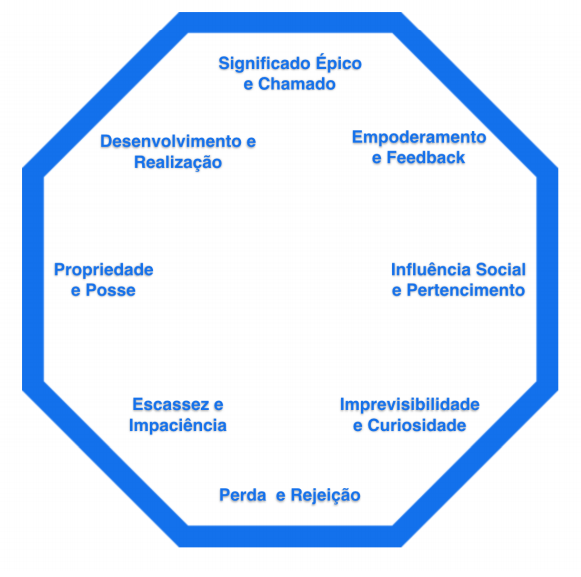
\includegraphics[width=300px, scale=1]{figuras/octalysisex}
    \caption{\textit{Octalysis Framework.}}
    \label{fig:octalysisex}
\end{figure}

Dentre as opções e os \textit{Frameworks} diferentes de gamificação, para a aplicação
deste trabalho é utilizado o Octalysis. Assim, é dedicado um capítulo
unicamente para a definição deste \textit{Framework}, que está disposto a seguir.

\section{\textit{Octalysis} Framework}
\label{sub:octalysisframework}
O \textit{Framework} \textit{Octalysis} foi desenvolvido pelo \cite{chou2015actionable} com a intenção de ser uma
base de auxílio para pessoas sem nenhuma capacitação sobre gamifição
conseguir definir e aplicar este processo em uma base qualquer.

Este Framework criado por \cite{chou2015actionable} possui várias mecânicas de funcionamento,
bem quanto à sua divisão tanto quanto à sua maneira de lidar com as
motivações básicas de casa usuário. Dessa forma, o subcapítulo a seguir
apresenta a forma com que o \textit{Octalysis} trabalha e quais são suas divisões básicas.

O Segundo subcapítulo diz respeito às fases do \textit{Octalysis}, bem como o último
apresentará uma estratégia de aplicação no cenário, já definida pelo próprio
\cite{chou2015actionable}.


\subsection{Mecânica do \textit{Octalysis}}
\label{sub:mecanicaoctalysis}
O funcionamento do Framework \textit{Octalysis} é subdividido em três partes, onde,
cada uma representa sua função específica. Essas três partes estão descritas
nas subsessões a seguir. A primeira trata sobre as definições de Motivações
Básicas, onde estas são dívidas em oito e cada uma tem sua função específica.
A segunda trata sobre a divisão direita e esquerda do Framework, onde cada
lado representa uma forma diferente de sentir diante certa ação.
A terceira e última trata sobre as definições de emoções, onde existem
pensamentos e sentimentos bons e por outro lado, sentimentos ruins.
Dessa forma, a seguir estão as próximas sessões.

\subsubsection{Oito Motivações Básicas}
\label{sub:oitomotivacoesbasicas}
As motivações básicas são ações que levam, motivam e engajam
o usuário para que este execute uma dada atividade alvo.
A diferença entre estas é que cada uma foca um tipo de sentimento
do usuário. Essas motivações contém um grupo de técnicas de \textit{game}
que podem ser aplicadas em um dado contexto para alcançar algum
objetivo. Dessa maneira, uma motivação básica nada mais é do
que um agrupamento de técnicas de gamifição separadas e agrupadas
por um sentimento que motiva o usuário.

Estas motivações básicas estão desenhadas dentro de uma figura para
compor uma organização. Esta figura contém oito pontas, por isso o nome:
\textit{Octalysis}. A figura \ref{fig:octalysisframework} represernta esta
disposição no diagrama.

\begin{figure}[h]
    \centering
    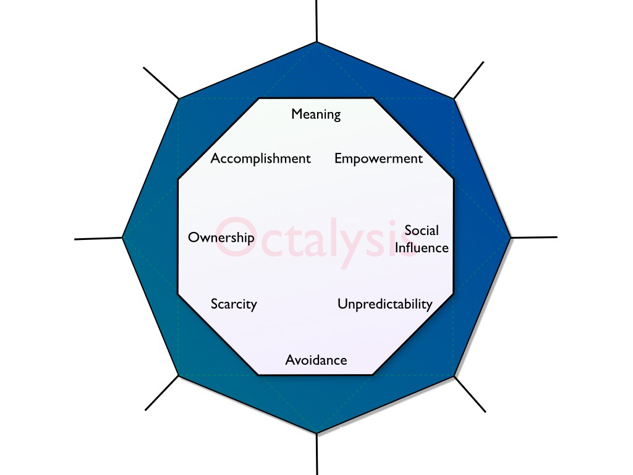
\includegraphics[width=400px, scale=1]{figuras/octalysisframework}
    \caption{\textit{Octalysis} Framework}
    \label{fig:octalysisframework}
\end{figure}

Dessa forma, a seguir, sãoexplicadas as oito motivações básicas,
apontando quais são as suas respectivas técnicas, bem como
suas devidas explicações.

\subsubsection{Significado Épico e Chamado}
\label{sub:significadoepico}
Esta motivação básica está em torno de fazer com que o usuário sinta que
está fazendo algo épico e ajudando a sociedade, sendo altruísta com toda
a população. Fazendo-o acreditar que pode mudar algo muito importante
na vida de várias pessoas. Projetos \textit{Open} \textit{Source} são uma clara evidência
disto, onde o desenvolvedor trabalha e contribui para a comunidade, ajudando
todos.

Também entra nesta fase o fato de um jogador entrar no jogo e ganhar um
privilégio aparentemente muito valioso. Onde este acredita que teve uma
oportunidade que nenhum outro jogador, acreditando que ganhou a sorte de
principiante.

A seguir estão descritos as técnicas desta motivação básica:

\begin{enumerate}
    \item Narrativa: uma história que se inicia ao começar um determinado
        jogo, colocando o usuário dentro do enrendo e aplicando o contexto
        do "\textit{Modus Operants}";
    \item Sorte de Principiante: sorte daquele que acredita que recebeu
        um benefício único e nenhum dos outros jogadores recebeu algo
        parecido;
    \item Lanche Grátis: técnica que atribui ou presenteia um dado usuário
        com algo que tem uma grande dificuldade de ser alcançado ou é
        caro e bastante dispendioso para o usuário.
        O ponto é que logo após o lanche, o \textit{game} o incentiva a tomar
        algumas ações definidas;
    \item Elitismo: é a ação de aumentar e incentivar atitudes de orgulho
        de um grupo, fazendo com que os usuários destes sintam-se
        únicos e privilegiados, a fim de assegurar o orgulho do
        grupo inteiro, fazendo com que todos os integrantes sintam-se assim;
    \item Héroi da Humanidade: vem da técnica de que o jogador pode e deve
        ajudar a quem não consegue se ajudar, fazendo com que este tome
        atitudes e ações em prol de uma causa muito maior.
\end{enumerate}

\subsubsection{Motivação Desenvolvimento e Realização}
\label{sub:desenvolvimentoerealizacao}
A motivação básica de Desenvolvimento e Realização traz como base fazer
com que o jogador seja desafiado, que ele tenha metas a cumprir e que este
tem que desenvolver habilidades e fazer progressos para que o desafio
seja superado. É importante que nessa fase tenha recompensas e ganhos para
o jogador, como troféus, medalhas, emblemas, entre outros, para que o
usuário entenda que todo o esforço do desafio não foi em vão e que
teve um objetivo de recompensa por ele.

Exemplos desta motivação são os pontos, medalhas, \textit{rankings}, tabelas de
classificação, emblemas, entre outros. Que já são largamente utilizados
em várias plataformas atualmente.

Alguns exemplos de técnicas de gamificação para a motivação básica
de Desafio e Realização estão listadas a seguir:

\begin{enumerate}
    \item Pontos: um esquema de pontos aplicado para mostrar o progresso
        de um jogador em qualquer ponto desejado do objeto a ser gamificado;
    \item Símbolos de conquista e realização: que são emblemas que podem
        ser utilizados como espécie de reconhecimento sobre dada
        atividade ou desafio que o usuário desempenhou. Estas podem ser
        medalhas, emblemas, troféus, uniformes, estrelas, entre outros;
    \item Tabelas de classificação: são tabelas que vão mostrar como o
        jogador se porta diante dos demais jogadores, como
        estão estes resultados e o quanto é necessário para alcançar
        algum determinado objetivo. Esta técnica pode ser aplicada através
        de \textit{rankings} e tabelas.
    \item Barra de Progresso: permite que o usuário tenha uma clara visão
        e um bom \textit{feedback} do quanto ele está cumprido ou cumpriu dentro
        de um determinado objetivo.
    \item Escolhas Óbvias: são caminhos diferentes onde o usuário tem que tomar
        uma certa decisão ou fazer uma escolha. Neste momento, o usuário tem um
        escolha óbvia dentre todas as demais. No momento que ele escolher a óbvia
        irá se achar inteligente por ter conseguido identificar algo e ter
        feito a escolha correta.
    \item Oásis no Deserto: é uma recompensa que está sugerida e presente logo
        após determinadas escolhas que o usuário pode fazer;
    \item Efeito Estrela do \textit{Rock}: faz com que o usuário se sinta importante,
        com a ideia de que todos que estão na rede estão com vontade de interagir
        com ele, fazendo com que este se sinta importante, uma estrela do \textit{rock}.
\end{enumerate}

\subsubsection{Motivação Empoderamento e Feedback}
\label{sub:empoderamentoefeedback}
A motivação básica de empoderamento e \textit{feedback} é expressada quando os usuários
estão engajados em algum processo criativo e eles tem que tomar ações repentinas
e tentar diferentes combinações.

Para esta motivação básica o usuário não precisa apenas saber expressar
sua criatividade de várias maneiras, porém, além disso, precisa ser capaz
de ver os resultados das suas criações e seus respectivos feedbacks.

As técnicas que guiam esta motivação básica são as que estão listadas
a seguir:

\begin{enumerate}
    \item Escolhas significativas: esta técnica está em torno de fazer
        com que o usuário, mesmo com várias opções de montagem,
        tome ações corretas. O caminho correto não precisa ser exatamente o mesmo,
        pode ser um quebra-cabeças que você monta como desejar e no final
        consegue alcançar o objetivo esperado;
    \item Etapa desbloqueada: o usuário consegue ter acesso
        e utilizar novas funcionalidades, com novas possibilidades
        assim que uma etapa for concluída;
    \item \textit{Boosters}: Itens temporários que o usuário tem alguma
        capacidade aumentada, com mais poder, durante um período
        determinado de tempo;
    \item Feedback instantâneo: característica que permite com que o usuário
        tenha uma resposta imediata das ações que ele escolheu fazer e proceder;
    \item Controle de tempo real: trazendo e possibilitando que o jogador
        possa controlar ações e opções de um determinado objetivo deste
        em tempo real;
    \item Chain Combos: um conjunto de ações que traz recompensa para o
        usuário, porém, quando feitos em seguida, como um combo, tem
        efeitos e ganhos maiores.
\end{enumerate}

\subsubsection{Motivação de Propriedade e Posse}
\label{sub:propriedadeeposse}
É a motivação que gira em torno de mostrar ao usuário e fazer com que
este acredite que ele tem posse sobre algo que está interagindo na
plataforma. Quando este, por exemplo, passa tanto tempo utilizando
ou personalizando algo que passa a sentir que aquele dado objeto
é propriedade dele.

Um exemplo que pode ser aplicado é a utilização de dinheiro e riquezas
virtuais, como moedas e \textit{bitcoins}. De toda forma, um acumulo de riquezas
em geral contempla esta técnica.

\begin{enumerate}
    \item Construir do zero: faz com que o jogador sinta que ele está
        fazendo algo do início, e não que está recebendo algo que
        já está pronto para que este trabalhe;
    \item Coleção: transmite a ideia de um conjunto de itens que se todos
        estiverem juntos e reunidos, este irá se sentir completo.
    \item Pontos permutáveis: faz com que o usuário consiga utilizar
        seus pontos para adquirir algo que é caro por padrão;
    \item Monitor \textit{Attachment}: faz com que o jogador sinta e tenha a
        sensação que é dono de algo devido ao longo monitoramento
        da atividade que está desempenhando;
    \item Efeito Alfred: este é definido quando os usuários
        sentem que um produto ou serviço é tão personalizado às
        suas próprias necessidades que não é possível fazer isso
        de nenhuma outra forma;
    \item Avatar: quando um jogador consegue criar um perfil que pode ser
        personalizado e permite com que este esteja próximo aos gostos e
        intenções do usuário.
\end{enumerate}

\subsubsection{Influência Social e Pertencimento}
\label{sub:influenciasocialepertencimento}
Esta motivação básica utiliza de elementos e fatos sociais de forma
a incentivar as pessoas à pensamentos e ações em grupos e comunidades,
de forma social.

Essa motivação básica vai de encontro com a característica de ver algum
amigo, conhecido ou familiar, que possui uma dado atributo ou expertise
em dada atividade. Você, rapidamente, analisando que não possui a mesma
habilidade, ou não no mesmo nível, se esforça e engaja para que consiga
alcançá-la e estar próximo de tal.

As técnicas que regem e que estão presentes na Influência Social e Pertencimento
são as listadas a seguir:

\begin{enumerate}
    \item Mentoria: no momento em que uma pessoa que possui mais experiência
        em um dado assunto e orienta aqueles que estão começando nesta, pode
        ser enquadrado nesta técnica;
    \item Vangloriar-se: mostrar e se apresentar aos demais usuários como
        alguém que possui uma determinada qualidade que é bem reconhecida
        por todos que estão em sua volta;
    \item Prateleira de Troféus: uma gama de troféus, recompensas e conquistas
        que estão bem aparentes para os demais usuários olharem e perceberem
        através de qualquer meio que foi estabelecido;
    \item Desafio em Grupo: dasafios que podem ser elaborados com ou dentro
        de um determinado grupo, que incentiva as pessoas a trabalharem
        em uma ação conjunta e não em algo isolado, com a utilização de atividade
        individual;
    \item Tesouro Social: são pontos, presentes e benefícios que podem ser atribuídos
        para você a partir de um determinado jogador ou amigo que se encontra dentro
        do círculo de amigos;
    \item Orgulho Social:  são ações pequenas, de pouco esforço, que auxiliam e contribuem
        para o convívio social, como eventos pequenos e pouco significativos,
        como um \textit{like} em uma determinada rede social, ou um compartilhamento;
    \item Âncora de Conformidade: esta técnica possui base no que já temos ciência
        através de nossa cultura;
    \item \textit{Water} \textit{Cooler}: esta técnica consiste em disponibilizar algum local
        aberto e comum para que as pessoas consigam escrever, expor e falar
        sobre fatos e atividades aleatórias, o qual agrada um determinado grupo.

\end{enumerate}

\subsubsection{Escassez e Impaciência}
\label{sub:escassexeimpaciencia}
Esta motivação leva o jogador a sentir-se ansioso e receoso com a espera de algo
que ele ainda não tem e para que consiga, tem que esperar por algum tempo.

Um exemplo bem utilizado deste ponto é a utilização dos \textit{games} por meio de dinâmicas
agendadas, onde esses dizem ao usuário para retornar dentro de determinado tempo.
E caso o jogador não queira esperar por este tempo, deve utilizar algo que é caro
para este.

Um exemplo disto é a aplicação do Facebook quando iniciou, que tinha um início que não permitia
que todos utilizassem a plataforma, apenas se houvesse um convite por parte de um
determinado conhecido que já está dentro da base.

As técnicas que regem esta motivação básica são as seguir:

\begin{enumerate}
    \item \textit{Dangling}: esta técnica deixa bem clara para o jogador que ele não pode
        ter algo que é bem gratificante. Que para ter deve esperar ou adquirir
        de uma forma cara e dispendiosa;
    \item \textit{Anchored} \textit{Juxtaposition}: esta técnica concede duas opções para o usuário.
        Uma delas custa dinheiro e a outra custa e exige bastante tempo e esforço
        por parte do usuário;
    \item \textit{Torture} \textit{Breaks}: esta técnica faz com que o usuário seja obrigado a esperar
        de qualquer forma para obter algo. Neste caso, existe um ponto em que
        se o usuário ficar por um período longo de tempo esperando esta ação
        utilizando o jogo, a gamifição já estará sendo bem aplicada;
    \item \textit{Evolved} UI: fazer com que as pessoas tenham poucas opções no começo da
        trajetória, porém, com o seu desenvolvimento, estas opções vão aumentando.
\end{enumerate}

\subsubsection{Imprevisibilidade e Curiosidade}
\label{sub:imprevisibilidadeecuriosidade}
Esta motivação básica gira em torno de envolver o usuário com atitudes e ações que são
imprevisíveis, que o usuário não tem noção sobre o resultado que poderá receber.

Isto faz com que o usuário permaneça com a mente ocupada cogitando o que poderá
acontecer com o evento imprevisível.

As técnicas que guiam esta motivação básica são as listadas a seguir:

\begin{enumerate}
    \item Ovo de Páscoa: esta é uma notícia ou surpresa que agrada o usuário,
        que nasce de uma ação que não é esperada;
    \item \textit{Mystery} \textit{Boxes}: são recompensas que podem ser qualquer coisa
        logo após que alguma ação ou evento for concluído;
    \item \textit{Visual} \textit{Storytelling}: fazer com que o usuário tenha informações
        advindas de formatos de livros e histórias
        visuais;
    \item \textit{Oracle} \textit{Effect}: esta técnica está em torno de fazer com que o
        jogador pense sobre o que está por vir, se é algo positivo ou não;
    \item \textit{Russian} \textit{Roulette}: é a prática onde de tempos em tempos algum dado ponto
        ou jogador deve ser penalizado.
\end{enumerate}

\subsubsection{Perda e Rejeição}
\label{sub:perdaerejeicao}
Esta motivação básica trabalha e se baseia em construir algo para que algo ruim não
aconteça com o jogador, ou seja, na prevenção de acontecimentos ruins.

São práticas como evitar que o jogador perca todas as atividades que desempenhou
até então, ou descobrir que todo o progresso foi em vão.

Estas atitudes motivam o usuário a executar determinados feitos com base no que
ele não quer que aconteça.

As seguintes técnicas ilustram como esses sentimentos são aplicados no meio:

\begin{enumerate}
    \item \textit{Reghtful} \textit{Heritage}: esta técnica está firmada em fazer com que o usuário
        acredite que algo é dele e pertence a ele, porém, depois de algum tempo,
        se o usuário não desempenhar determinadas ações, este terá este ponto
        perdido;
    \item \textit{Evanescente} \textit{Opportunities}: algo que não vai aparecer jamais
        caso o usuário não tome uma ação requerida rapidamente;
    \item \textit{Countdown} \textit{Timers}: são esquemas de contagem regressiva para determindas
        atividades, que tem um tempo máximo para se concluir;
    \item \textit{Status} \textit{Wuo} \textit{Sloth}: tendência de mostrar ao jogador que este não irá evoluir ou melhorar se continuar
        a tomar atitudes como estão sendo tomadas;
    \item \textit{FOMO} \textit{Ponch}: este é um ponto muito forte da Motivação Básica 8, que tem como
        pretexto gerar no jogador um medo de perder, seja já qual for o que
        este adquiriu.
\end{enumerate}

\subsubsection{Lado Esquerdo e Direito do Cérebro}
\label{sub:leftright}
O \textit{Octalysis} \textit{framework} está dividido em duas partes, tais quais o \cite{chou2015actionable} nomeia
de \textit{Left Brain e Right Brain}, sendo que cada um destes é correspondente com qual lado do cérebro
as técnicas vão atuar. Cada motivação está posicionada em um dado local, que
representa um pensando de uma dada forma ou o contrário. Este posicionamento
da MB em cada lado representa qual lado do cérebro é utilizado.

A figura \ref{fig:octalysisleftright} ilustra esta divisão entre as técnicas.

\begin{figure}[h]
    \centering
    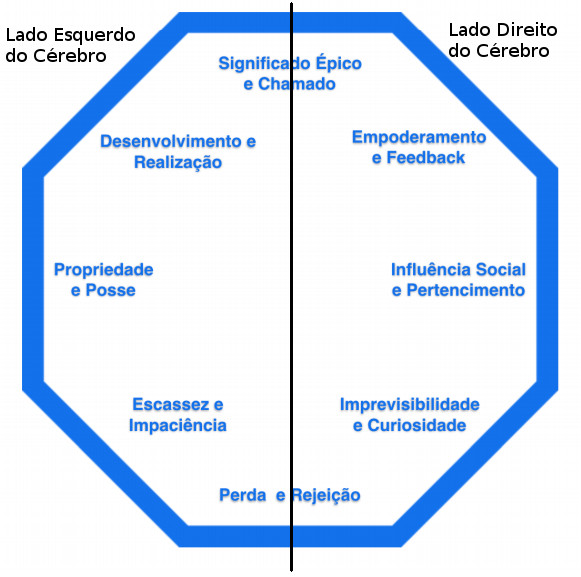
\includegraphics[width=400px, scale=1]{figuras/octalysisleftright}
    \caption{\textit{Left Brain and Right Brain}}
    \label{fig:octalysisleftright}
\end{figure}

Pode ser visto que existem técnicas do lado direito e do lado esquerdo. As
motivações básicas do lado direito estão mapeadas também com o lado direito
do cérebro, o qual tem ligação com as atividades lógicas, de raciocínio lógico.
Já as motivações básicas do lado esquerdo represetam ações mais criativas,
sentimentais e imprevisíveis.

\subsubsection{Sentimentos bons e ruins}
\label{sub:whiteblack}
As motivações básicas estão muito ligadas à característica de pensamento e
sentimento que é gerado no jogador. Cada motivação básica gera um tipo de
sentimento e vontade diferente no usuário.

Estas diferenças são representadas pela parte superior, representadas
pela \textit{White Hat}, que são sentimentos e motivações boas, que trazem
boas impressões para o jogador. A divisão é feita exatamente como
foi explicada na sessão \ref{sub:leftright}, porém, agora a
divisão é feita entre a parte superior ou inferior do \textit{framework}.

Porém, a parte inferior do \textit{framework} representa sentimentos ruins, que o jogador
vem a sentir no momento que participa e utiliza determinada MB. Já a
parte superior representa boas motivações, que ele chama de \textit{White Hat}.

Todas essas disposições podem ser vistas na figura
\ref{fig:octalysiswhiteblack} a seguir.

\begin{figure}[h]
    \centering
    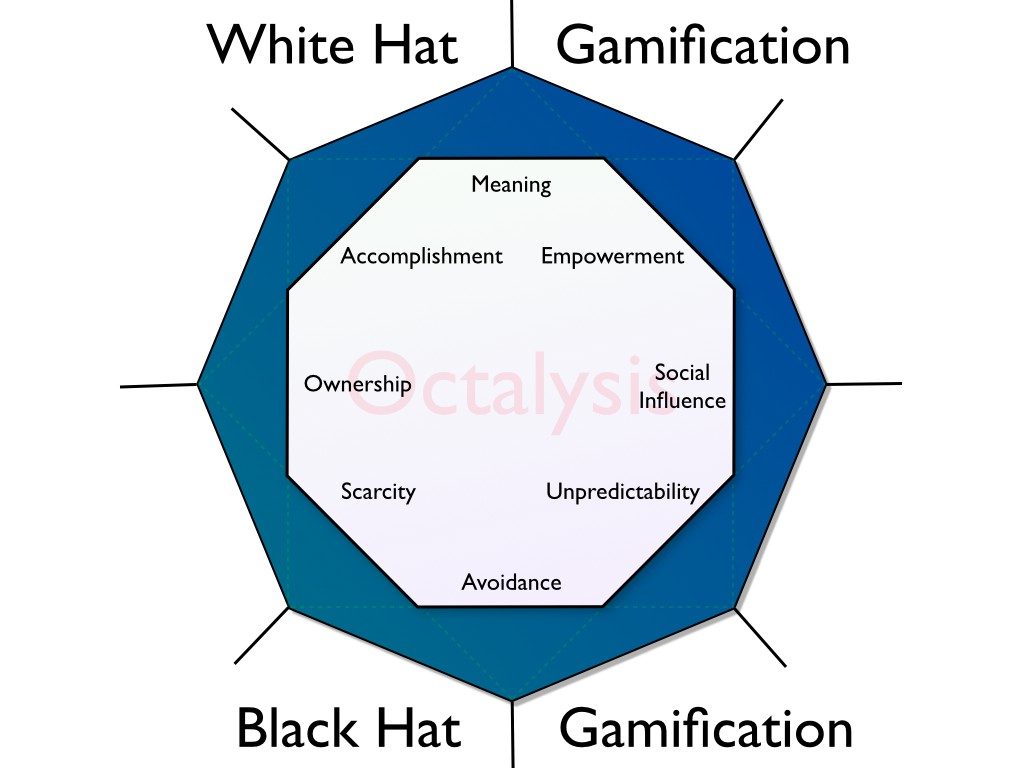
\includegraphics[width=400px, scale=1]{figuras/octalysiswhiteblack}
    \caption{\textit{White Hat and Black Hat}}
    \label{fig:octalysiswhiteblack}
\end{figure}

\subsection{Fases da Gamificação}
\label{sub:fasesgamifição}
Todos os produtos que as pessoas utilizam na internet possuem diferentes
fases ao longo do seu ciclo de vida. Cada fase é reponsável por um tipo de contato diferente
do usuário com a interface e com a imersão em que este está submetido.

Cada fase representa um sentimento diferente, uma experiência diferente
e uma nova forma de se lidar com aqueles atributos referentes ao que está
em escopo no procedimento de interação com o produto propiciado.

Essas fases que cada projeto é submetido já são conhecidas e desenhadas. As fases
são quatro, bem claras e definidas. Elas são as seguintes:

\begin{enumerate}
    \item Descoberta;
    \item Reconhecimento;
    \item Construção;
    \item Fim de jogo.
\end{enumerate}

Essas fases circundam o ciclo de vida de um produto, desde o momento que este
é apresentado ao público até o momento que é deixado por ele.

A definição das fases é ilustrada claramente nos subcapítulos que virão a seguir.

\subsubsection{Descoberta}
\label{sub:descoperta}
É a fase onde o usuário não conhece sobre o produto, não tem noção de quais são
os
seus objetivos nem como pode utilizá-lo. Esta é a fase onde o usuário tem o primeiro
contato, onde percebe como este funciona, bem como seus conceitos e valores.

Um exemplo de descoberta é uma apresentação de uma página no facebook, onde,
o novo produto é demonstrado para grupos e nichos de interesse. A partir
de então, o usuário poderá passar a conhecer e utilizar o sistema.

Resumidamente, esta fase é reponsável por aprensentar o produto, fazer
com que os usuários o conheça.

\subsubsection{Reconhecimento}
\label{sub:reconhecimento}
Esta fase é reponsável por demonstrar ao usuário como o sistema se comporta.

Ela é essencial para que este entenda como o sistema funciona e o que cada
componente executa. Um exemplo bem conhecido desse procedimento é a utilização
de tutoriais e guias para novos usuários, no momento da sua chegada.

Ela termina quando o usuário está apto a continuar a utilizar o site sem
necessidade de aprender muitas outras novas ferramentas e funcionalidades.

Quando este está apto para tal, inicia-se a maior fase, onde o usuário
vai de fato entender e conhecer sobre o procedimento que está lidando.

\subsubsection{Construção}
\label{sub:constru_o}
Esta é a fase responsável pela real utilização do produto, onde as \textit{features}
de fato são utilizadas e irão agregar valor ao usuário.

Nesta parte o usuário já sabe e entende o papel de cada funcionalidade. Ele é capaz
de atingir os objetivos propostos. Aqui os recursos propostos são utilizados
a depender na experiência e conexão do usuário com o produto.

Aqui tem que ser criados gatilhos para que mantenha o usuário constantemente utilizando
o sistema de acordo com o planejado.

\subsubsection{Fim de Jogo}
\label{sub:fim_de_jogo}
Toda aplicação desenvolvida passa pela fase de partida, onde é totalmente utilizada
e de alguma forma, o usuário a deixará.

Não necessariamente deixará de utilizar e participar do envolvimento total proposto pela
organização. Um exemplo disto é um jogo desenvolvido. Quando o primeiro jogo acabar, o
usuário passará pela fase de fim de jogo, que pode deixar o usuário motivado a se conectar
e adquirir a próxima versão do jogo que é lançada futuramente.

É importante que seja feito corretamente o desfeixo do produto para que uma linhagem seja
prosseguida.


Todas essas diretivas e fases que existem dentro do ciclo de vida de um produto
devem ser
tratadas de forma independente e diferente entre si. Agora pode-se indagar onde
a gamificação
entra neste processo, sendo que cada fase deve ser tratada de uma forma diferente pelo
usuário e, consecutivamente, por parte de quem está a oferecer o produto.

Assim, há a necessidade de que a gamificação também seja moldada conforme o objetivo de
cada fase a ser aplicada.

Dessa forma, cada fase implementada é pensada e avaliada para que seja possível
aplicação de um  projeto de gamificação. Cada fase terá um foco em motivações
básicas diferentes, que propiciarão uma experiência diferente para o usuário.

A figura \ref{fig:fasesoctalysis} ilustra um exemplo do como pode ser aplicado na
Rede Social About a gamificação ao longo das quatro fases.

\begin{figure}[h]
    \centering
    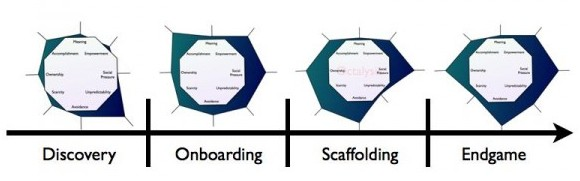
\includegraphics[width=400px, scale=1]{figuras/fasesoctalysis}
    \caption{Fases do \textit{Octalysis}}
    \label{fig:fasesoctalysis}
\end{figure}

Como pode ser visto na figura \ref{fig:fasesoctalysis}, são projetados vários
desenhos e \textit{designs} modificados e diferentes para cada fase. Cada uma destas
tem um pensamento e objetivo diferente.

Na fase de descoberta, pode ser visto que a motivação básica mais presente é
a imprevisão e a curiosidade. O que dá margem para que o usuário imagine diferentes
possibilidades sobre o produto.

No momento de uma propaganda, por exemplo, este lado do \textit{framework} pode gerar uma
extrema curiosidade no usuário, o que fará com que ele fique motivado a procurar
e entender mais sobre o que está sendo anunciado.

Isto pode ser extremamente importante para conseguir capturar novos usuários.

Na segunda fase, em que o usuário vai conhecer sobre o produto, pode ser visto
que as fases relativas a desenvolvimento próprio e realização de si mesmo
são bem mais presentes.

Este ponto pode ser aplicado, pois o usuário irá se sentir realizado e inteligente
ao observar seu desenvolvimento próprio elevado. Isto irá gerar um prazer em fazê-lo
sentir o quanto pode ser bom em realizar as tarefas que a ele estão sendo designadas
no início do procedimento.

Na terceira fase é possível verificar que duas motivações básicas são muito presentes:

\begin{itemize}
    \item Motivação Básica Cinco: Influência e Dinâmica Social;
    \item Motivação Básica Seis: Escassez e Impaciência.
\end{itemize}


Para a Motivação Básica Cinco, isto deixa o usuário motivado ao utilizar o produto
por sentir que está exercendo uma alta influência social, que está envolvido em
uma dinâmica social que faz influência em outras pessoas.

Isto faz com que o usuário fique motivado a continuar engajado no processo, pois
este estará conseguindo perceber o quanto está sendo participativo no meio social
e que o produto está sendo proveitoso por fazê-lo se sentir socialmente influente
e participativo.


A segunda motivação básica vizualizada nesta fase, Escassez e Impaciência, acontece
pois é possível verificar que o usuário fique motivado a executar determinadas
tarefas baseado neste sentimento.

Esta o deixará preocupado com a questão de não cumprir corretamente os objetivos.
Esta fase é responsável por fazê-lo se sentir em um meio escasso caso não execute
os objetivos propostos.

Isto vai motivar o usuário e vai fazer com que faça o necessário para que não
sinta estes sentimentos.

A última fase, fim de jogo, também tem sua motivação básica predominante que
a guia. Esta é guiada pela Motivação Básica Oito: perca e rejeição.

Esta irá gerar um sentimento que faz o usuário se sentir mal. Este sentimento
envolve o fato de que o usuário pode perder todo o processo que foi executado.



Este é um sentimento ruim. Sentimento qual o usuário não deseja sentir. Para tanto
ele se esforçará a fim de não presenciar as experiências que são submetidas.

Como pode ser visto, estes procedimentos de cada fase são extremamente aplicáveis
e úteis para que o usuário tenha várias experiências ao longo do clico de vida do
produto. O que propiciará uma experiência muito mais agradável.

Dessa forma, são desenhados quatro frameworks diferentes para a Rede Social About.
Uma para cada fase diferente do produto, onde são estudadas separadamente para
aplicá-las e possibilitar uma boa experiência para o usuário.

\subsection{\textit{Octalysis Strategy Dashboard}}
\label{sec:octalysisdashborad}
O \textit{framework} \textit{Octalysis} oferece suporte para a construção de um projeto de gamificação
bem estruturado e baseado em necessidades do domínio do problema.

Este suporte se trata do \textit{Octalysis} \textit{Strategy} \textit{Dashboard}, o qual pode ser analisado
 as
estretégias de mercado, perspectiva do usuário, intenções desejadas para a gamificação,
mecanismos de \textit{feedback} e incentivos.

Existem processos sistematizados para estabelecer cada fase e como é dado o
resultado da gamificação.

Para este trabalho, são utilizados estes procedimentos sistematizados.

Para ilustrar a metodologia de estratégia do \textit{Octalysis} \textit{dashboard}, é representada
a figura a seguir, que contém a metodologia e a formalização da sua construção.

A seguir são descritos subcapítulos, que retratarão o papel e a utilidade de
cada
componente.


 \begin{figure}[h]
     \centering

     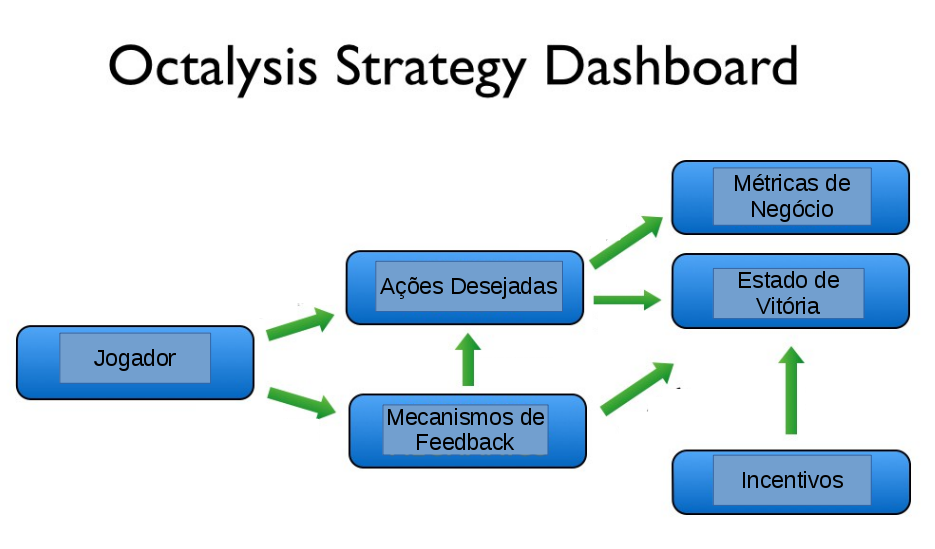
\includegraphics[width=450px, scale=1]{figuras/dashboard}
     \caption{\textit{Octalysis} \textit{Strategy} \textit{Dashboard}}

     \label{fig:dashboard}
 \end{figure}

\subsubsection{Métricas de Negócio}
\label{sub:business_metrics}
As métricas de negócio, são termos quantitativos que podem ser utilizados
para ter um número palpável sobre como está um determinado ponto do projeto de gamificação
que teve como o objetivo de ser atacado.

Essas métricas, irão auxiliar a verificarmos o quanto a aplicação da gamificação
 foi eficaz ou
não dentro de um determinado objetivo.

Alguns exemplos de técnica de gamificação que são utilizadas estão a seguir:

\begin{itemize}
    \item Aumentar o número de seguidores dos usuários prêmio;
    \item Aumentar o número de vendas de um livro sobre o produto;
    \item Aumentar o número de inscritos na rede social;
    \item Aumentar a quantidade de acessos diários;
    \item Aumentar os seguidores inscritos;
    \item Aumentar os usuários que compartilham conteúdos pelas redes sociais;
    \item Aumentar a quantidade de curtidas em determinado post.
\end{itemize}

Estes exemplos de métricas são submetidos à Rede Social About antes da apresentação da
gamificação. E assim que determinada técnica for utilizada, é então executada
 uma
segunda medição, que propiciará analisar as diferenças entre os resultados obtidos.

\subsubsection{Definir Tipos de Usuário}
\label{sub:define_user_types}
Este ponto do \textit{dashboard}, para definir os tipos dos usuários, é responsável por conseguir
elaborar e definir quais são os tipos de usuários que são almejados e trabalhados, quando
falamos sobre gamificação.

Esta fase é um processo de definição de nicho sobre onde a gamificação vai atuar, quanto a
usuários, dentro da Rede Social About? Quais são os passos utilizados para que este público
seja atingindo?

Alguns exemplos de tipos de usuário se encontram a seguir:

\begin{itemize}
    \item Companhias que desejam que seus trabalhadores atinjam determinadas métricas
        ao fim de cada mês;
    \item Educadores e políticos que querem utilizar conhecimento para criar impactos
        sociais;
    \item Indivíduos que são apaixonados por gamificação, \textit{games} e desenvolvimento próprio.
\end{itemize}

Desta maneira, é possível realizar um projeto de gamificação focado ao definir o tipo
de usuários. Pois, a partir daí, é possível identificar quais caminhos são mais vantajasos
quanto a escolha das motivações básicas que são utilizadas ao longo das quatro fases.

\subsubsection{Definir Ações Desejadas}
\label{sub:define_desired_actions}
A definição das ações desejadas são todas as iniciativas tomadas pelo usuário que o levam a caminhar para
o \textit{Win} \textit{Stade} (Estado de Vitória), seja ela em qual fase for. Sendo assim, a Rede Social
About terá alguns pontos que são definidos como os desejados. Estes são desenhados
até que o estado de vitória seja definido. Assim, para as quatro fases são definidas
ações diferentes. Alguns exemplos de ações que podem ser escolhidas são apresentadas
a seguir.

Ações na fase da descoberta:
\begin{itemize}
    \item Conhecer a Rede Social About;
    \item Clicar no link da Rede Social About;
    \item Conhecer as \textit{features} oferecidas pela Rede Social.
\end{itemize}


Ações na fase de reconhecimento do projeto:
\begin{itemize}
    \item Executar o tutorial de uso da About;;
    \item Compartilhar a Rede Social About com os amigos;
    \item Adicionar foto e email na \textit{network};
    \item Permitir a inscrição na lista de email.
\end{itemize}

Já para a fase de construção do projeto, os seguintes pontos podem ser um
exemplo:

\begin{itemize}
    \item Fazer login diariamente na \textit{network};
    \item Abrir semanalmente os emails enviados pela \textit{network};
    \item Compartilhar abouts com os amigos;
    \item Participar de grupos no facebook sobre a rede social about;
    \item Adquirir a versão prêmio da rede social about;
    \item Inscrever em grupos de discussão sobre a rede social about;
    \item Escrever mais de um about diariamente;
    \item Votar em mais de vinte abouts diários.
\end{itemize}

Por fim, na fase de fim de jogo, alguns exemplos de construção podem ser dados.
Eles são os seguintes:
\begin{itemize}
    \item Se tornar contribuidor da Rede Social About;;
    \item Fazer parte da equipe de desenvolvedores da About;
    \item Propor melhorias para a about;
    \item Tornar-se moderador dos abouts.
\end{itemize}

Estes exemplos ajudam e esclarecer como os objetivos podem ser alcançados. Elas
definem um nível de
granularidade maior.

\subsubsection{Definir Mecanismos de \textit{Feedback}}
\label{sub:define_feedback_mechanics}
A definição de mecanismos de \textit{feedback} são extremamente importantes para a experiência do usuário
com a \textit{network}. Este é responsável por ilustrar e deixar bem claro para o usuário
, como ele está
prosseguindo no desenvolvimento do projeto.

Atualmente os usuários tem requirido feedbacks constantes, em tempo real, para as suas ações
realizadas. Sendo assim, é necessário que existam esses gatilhos em vários pontos da
Rede Social About e que o usuário possa entender rapidamente.

A seguir estão alguns exemplos de como podem ser esclarecidos esses feedbacks para o usuário:

\begin{itemize}
    \item \textit{Countdown} \textit{Timers};
    \item Desbloquear conteúdo da página;
    \item Status de progresso na \textit{sidebar};
    \item Verificação de qual era a melhor escolha;
    \item Vídeo embutido;
    \item Barra de pontos de status;
    \item Certificados;
    \item Medalhas;
    \item Gráficos de desempenho.
\end{itemize}

Assim, com exemplos dessa maneira, é possível que o usuário verifique o quanto suas atividades estão
sendo aproveitadas.

\subsubsection{Incentivos e Recompensas}
\label{sub:incentives_and_rewards}
O sistema de incentivos e recompensas fecham o ciclo do \textit{dashboard}, que fazem com que
os usuários se sintam motivados a alcançar cada estado de vitória. Eles ajudam a
indicar
o quanto ainda falta para que o estado seja almejado.

\begin{itemize}
    \item \textit{Status} \textit{Points}
    \item Símbolos de vitórias;
    \item Conhecer os desenvolvedores da about;
    \item Ter acesso a arquivos confidenciais;
    \item Descontos nos produtos.
\end{itemize}

\subsubsection{Objetos de Gamificação}
\label{sec:objetodegamificacao}
Os objetos de gamificação são os pontos da rede social em que é aplicado o \textit{framework},
com os objetivos de atingir alguma meta de negócio.

Os objetivos de gamificação são os seguintes:

\begin{itemize}
    \item Fazer com que o usuário escreva mais abouts;
    \item Fazer com que o usuário julgue mais abouts;
    \item Fazer com que o usuário convide amigos que não estão cadastrados na about.
\end{itemize}



\section{Redes Sociais}
\label{sec:redessociais}
As redes sociais, ou cunhando o termo em inglês: \textit{Social} \textit{Network} \textit{Sites}(SNSs),
tem se tornado extremamente populares na última década. 
Várias
Redes Sociais despontaram e tomaram proporções grandes, tendo uma gama grande
de usuários participando destas. Alguns exemplos são: \textit{MySpace}, \textit{Facebook}, \textit{Twitter},
\textit{ByWorld}, entre outras, que conseguiram milhões de usuários, onde a maioria integra
as suas funcionalidades com hábitos diários praticados pelos usuários.
Estas redes sociais estão repletas de tecnologias e funcionalidades diferentes,
trazendo características e suportando uma gama grande de interesses e práticas
entre as pessoas. Na maioria das vezes, apoiado na persuasão e na presença social
dos indivíduos. Estas informações e a definição de rede social é defendida por
\cite{socialnetworkdefinition}, os quais serão propostos nas próximas sessões.
\subsection{Definição de Rede Social}


\label{sec:definicao}
Para \cite{socialnetworkdefinition}, um site de rede social é um serviço
de base \textit{web}, que permite que usuários individuais construam um perfil público, ou
semi público definido pelas fronteiras do sistema. Este articula com uma lista de
vários outros usuários com quem podem compartilhar uma conexão, além de ver e
interagir com esta gama. Estes podem fazer novos amigos e novas conexões no sistema.
Assim, tem-se que a natureza da própria nomeclatura induz que essas ligações
são elaboradas e modificadas de um site para outro, sendo que cada um tem a sua
peculiaridade.

Este defende que uma rede social não é única devido as suas características individuais,
que são diferentes ou estranhas perante às demais, pois esta capacidade é facilmente
contornada e copiada por outras bases. Mas o que faz com que uma SNS seja única
é a gama de usuários que estão ativamente utilizando a plataforma e as articulações
entre eles, bem como o que pode ser visto pelas demais pessoas com quem ele está
interagindo.

\subsection{História das Rede Sociais}
\label{sec:historiadasredessociais}
Anah e Ellison projetaram uma timeline, entre os anos de 1997 e 2006, que mostra
quando determinada rede social foi lançada ou relançada. Ela pode ser observada
na figura \ref{fig:historicosns}.

\begin{figure}[h]
    \centering
    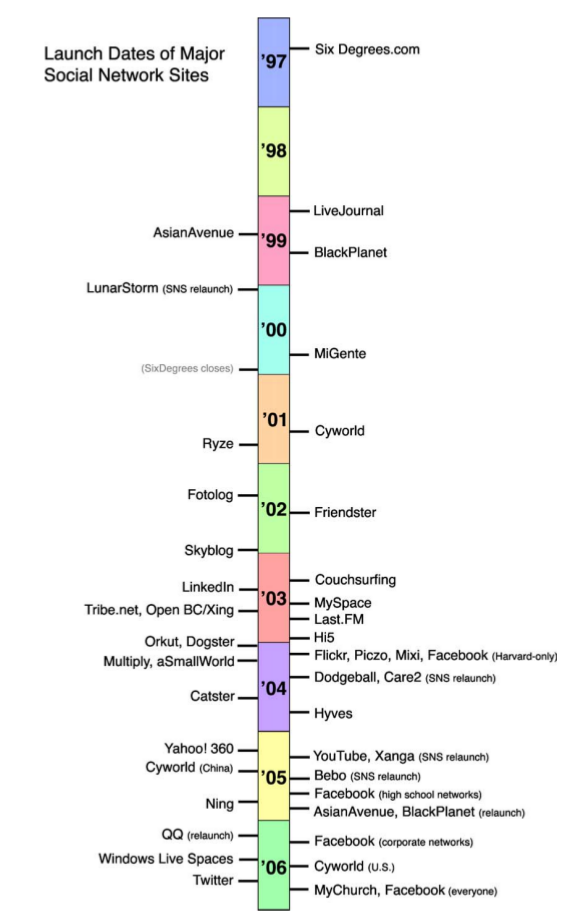
\includegraphics[width=330px, scale=1]{figuras/historicosns}
    \caption{\textit{Timeline of the launch dates of many major SNSs and dates when community sites
re-launched with SNS features. }}
    \label{fig:historicosns}
\end{figure}

Pode-se observar, de acordo com a timeline, que a primeira rede social que se tem
registro, utilizando o conceito abordado acima, é a \textit{SixDegrees.com}, sendo lançada
em 1997. Esta permitia com que os usuários criassem seus perfis, que adicionassem
amigos, tendo assim uma lista destes. E em 1998, começou a permitir que fosse possível
navegar entre os perfis que estavam em sua lista de amigos. Segundo os autores,
essas características e vizualização de perfil já existiam antes mesmo da \textit{SixDegrees.com,}
em várias aplicações de encontro romântico que eram presentes.

Em 1999, \textit{LiveJournal} adicionou algo que se tornaria muito comum nos dias de hoje:
a lista de conexões com outros amigos dos seus amigos em suas respectivas páginas.
Além disso, ela propiciava com que os usuários conseguissem marcar os amigos
dos seus amigos como conexões diretas, para que estes conseguissem ver seus Jornais
publicados, além disso, era possível fazer a gerência de privacidade, para
aplicar filtros e informações que os usuários poderiam ver.

A próxima onda de redes sociais começaram com a \textit{Ryze.com}, que foi lançada em 2001,
para ajudar as pessoas a alavancarem as suas carreiras pela internet, similar
ao que temos no LinkedIn nos dias de hoje. O fundador da \textit{Ryze} disse que mostrou o site à seu amigo,
e alguns laços foram criados, primeiramente na cidade de São Fransisco. Para este
escopo eram utilizados apenas alguns negócios de tecnologia e comunidades acadêmicas
incluindo entusiastas e investidores de informática para esta SNS. No final das
contas \textit{Ryze} nunca atingiu uma popularidade grande e posteriormente a \textit{Tribe.net} foi mais atrativa para o
público neste nicho de negócio, logo após, sendo substituída pela atual \textit{LinkedIn}.

Um grande investimento começou a ser aplicado no Vale do Silício, e várias pessoas
começaram a virar as suas atenções para produtos desenvolvidos ali. Um dos exemplos
de sucesso, foi o Google Orkut, que em 2006 foi  um fracasso nos Estados Unidos, porém
sofreu uma invasão brasileira, que fez com que este se tornasse uma forte potência
nacional. Outros exemplos deste local foram os espaços \textit{Live} da \textit{Microsoft}, como a.k.a. \textit{MSN}.

O \textit{MySpace} começou a ser desenvolvido em Santa Mônica, na Califórnia no ano de 2003.
Os seus fundadores tinham uma estratégia de conseguir conquistar os usuários de uma
outra plataforma já conhecida, a  \textit{Friendster}. O \textit{MySpace} conseguiu com algum tempo
tomar o mercado e se consagrou, em 2007, como uma grande potência nos Estados Unidos.

Porém, enquanto o \textit{MySpace} estava dominando o território americano, outras redes sociais
estavam desbravando o mundo, como \textit{Orkut}, aqui no Brasil e na Índia, \textit{Mixi} no Japão, 
\textit{Lunar} \textit{Storm} na Suécia, \textit{Dutch} na Polônia dentre vários outros exemplos. Por sua vez, nascia
no ambiente acadêmico o \textit{Facebook}, em 2004, apenas para a \textit{Harvard}. Em 2005, o \textit{Facebook} começou
a ser difundido para estudantes de universidades americanas e profissionais corporativos.

Com um grande investimento de alguns visionários, o \textit{Facebook} se tornou uma grande empresa
com potenciais mundiais, como é o caso hoje, e está presente em vários países espalhados
pelo mundo.

\subsection{Redes Sociais Anônimas}
\label{sec:redesociaisanonimas}
No ambiente das redes sociais, existem vários escopos e tecnologias de desenvolvimento.
Ou seja, existem muitas redes sociais que abordam várias categorias diferentes
de SNS. Uma dessas linhagens são as redes sociais que tem alguma característica
anônima, tendo um caráter de mistério sobre os fatos relatados. Serão
abordados dois exemplos de redes sociais anônimas: \textit{ExpressMind} e \textit{Social Matching.}

O estudo da \textit{Social Matching,} realizado por \cite{expressmind},
apresenta os resultados desta. Ela trazia uma série de indicações para o usuário,
possibilitando executar as opções de afirmar se gosta ou não de peculiaridades
destes. Assim, o sistema tem algoritmos de \textit{match} para verificar quais são
os potenciais \textit{matches} e os indicando aos usuários. Eles tiveram um bom resultado,
apontando um resultado final de 33\% mais \textit{matches} com a utilização do algoritmo
do que sem este.

Outro estudo, abordando as funcionalidades e funcionamento da \textit{ExpressMind},
produzido por \cite{expressmind}. Esta tinha a funcionalidade
de  permitir com que os usuários façam posts anônimos, não mostrando id, label ou nenhuma
maneira de fazer com que os leitores leiam sobre o que foi postado. Isto faz com que os
usuários possam falar sendo imparciais, gerando maior liberdade para
seus anúncios.

Uma outra \textit{feature} presente na \textit{ExpressMind} é o sistema de recomendação e atribuição
de notas aos posts e aos usuários. Este sistema de recomendação possui notas
de -5 a +5, sendo que tanto os usuários quanto os posts possuem esta nota.

Essas notas são utilizadas como entrada para os algoritmos de recomendação e
\textit{ranking} dos usuários e posts. Que formam uma lista das relações entre
os usuários.

\cite{expressmind} fizeram uma pesquisa com seus usuários
para avaliar quais motivos faziam com que cada um estava utilizando a rede social. 
O resultado está na figura \ref{fig:expressmind}.


\begin{figure}[h]
    \centering
    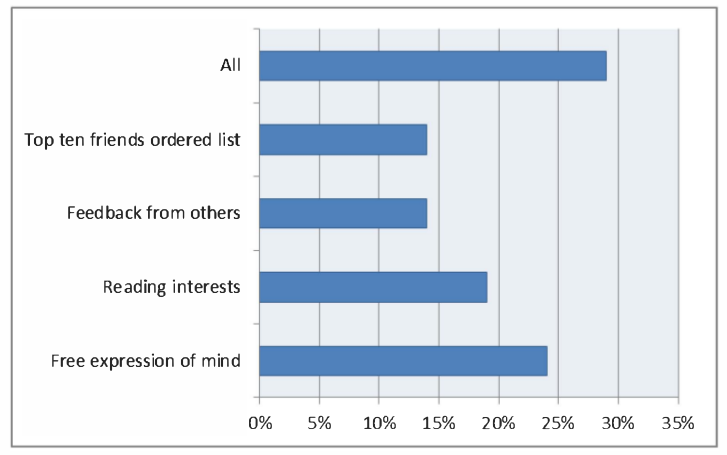
\includegraphics[width=330px, scale=1]{figuras/expressmind}
    \caption{Em quais são as propriedades da rede social que os usuários estão interessados?}
    \label{fig:expressmind}
\end{figure}

Com estes resultados, dentre as opções avaliadas separadamente, é possível
observar que a principal motivação que fazem os usuários utilizarem a rede social \textit{match}
é a possibilidade de expressão livre, onde o usuário pode expressar seus sentimentos
e suas vontades bem com este se interessar.

Este é um ponto que a proposta deste trabalho abrange fortemente, possibilitando que
as pessoas expressem o que pensam livremente sobre outras. Desta maneira,
estes pontos serão abordados ao longo do desenvolvimento da Rede Social About.

\section{Desenvolvimento de \textit{Software}}
\label{sec:processo_de_desenvolvimento_de_software}
Este capítulo apresenta conceitos sobre processos de produção de \textit{Software} e alguns modelos de processo genéricos, como cascata, evolucionário e outros.

\cite{pressman2009engenharia} traz uma boa definição para processos de \textit{Software}, afirmando que trata-se de um conjunto de metodologias definidas das atividades, ações e tarefas definidas para o desenvolvimento de um \textit{Software} de alta qualidade.

A Engenharia de \textit{Software} (ESW) está diretamente ligada com o processo. Seu compromisso é garantir que haja qualidade de produção, pois, qualidade do processo resulta em qualidade no produto.

De acordo com \cite{pressman2009engenharia}, os engenheiros de \textit{Software} tem que possuir criatividade e conhecimento para que sejam capazes de analisar a demanda do mercado e então alinhar o desenvolvimento da melhor maneira possível, para que o resultado seja um produto de qualidade e entregue no prazo de tempo esperado.

 Para detalhar um processo, \cite{pressman2009engenharia} diz que um procedimento de \textit{Software} consiste em definir qual metodologia será utilizada para executar as diversas ações que o compõem. Além disso, as ações são um conjunto de tarefas de trabalho a ser completadas, artefatos de \textit{Software} que serão produzidos, marcos utilizados para indicar estado do processo e fatores para garantir a qualidade.

Para \cite{sommerville2011software}, existem muitas metodologias diferentes para se desenvolver um \textit{Software}, porém, algumas atividades são fundamentais para qualquer desenvolvimento, dentre elas são citadas as seguintes:

\begin{enumerate}
    \item Especificação de \textit{Software}: é preciso definir a funcionalidade do \textit{Software} e as restrições em sua operação;

    \item Projeto e implementação de \textit{Software}: deve ser produzido o \textit{Software} de maneira que cumpra a especificação;

    \item Validade de \textit{Software}: o \textit{Software} precisa ser validado para garantir que ele faz o que o cliente quer que seja feito;

    \item Evolução de \textit{Software}: o \textit{Software} precisa evoluir para atender as necessidades mutáveis do cliente.
\end{enumerate}


\cite{sommerville2011software} afirma que um modelo de \textit{Software} é uma representação de um processo de forma abstrata. Existem vários modelos genéricos de produção de \textit{Software}, e que podem ser adaptados. Porém alguns podem ser destacados:

\begin{itemize}
    \item Modelo em cascata: este modelo considera as atividades de especificação
        , desenvolvimento, validação e evolução que são fundamentais para 
        o processo, e as representa como fases separadas do processo, como 
        a especificação dos requisitos, projeto do \textit{Software}, implementação, testes e assim por diante;

    \item Desenvolvimento evolucionário: essa abordagem intercala as atividades 
        de especificação, desenvolvimento e validação. Um sistema inicial 
        é rapidamente desenvolvido a partir de especificações abstratas, 
        que são então refinadas com informações do cliente, para produzir 
        um sistema que satisfaça suas necessidades;


    \item Desenvolvimento formal de sistemas: essa abordagem se baseia 
        na produção de uma especificação formal de matemática do sistema 
        na transformação dessa especificação, utilizando-se de métodos 
        matemáticos para construir um programa. A verificação de componentes 
        do sistema é realizada mediante argumentos matemáticos, mostrando 
        que eles atendem as suas especificações;

    \item Desenvolvimento orientado a reuso: essa abordagem tem como base 
        a existência de um número significativo de componentes reutilizáveis.
        O processo de desenvolvimento de sistemas se concentra na integração 
        desses componentes em um sistema, em vez de proceder o desenvolvimento 
        a partir do zero.

\end{itemize}

Dentre esses quatro modelos, étratado neste trabalho o modelo de desenvolvimento 
evolucionário. Pois as metodologias ágeis, metodologia foco deste estudo
, se enquadra neste modelo


Dessa maneira, são apresentados conceitos sobre as metodologias de desenvolvimento ágil, bem como algumas filosofias abordadas por ela.
As metodologias de desenvolvimento ágeis podem ser expressadas por uma agregação de princípios e valores, onde buscam priorizar o seguinte conjunto de valores, de acordo com \cite{beck2001agile}, descritos no Manifesto para o Desenvolvimento Ágil:


\begin{itemize}
    \item Indivíduos e interações mais que processos e ferramentas;
    \item \textit{Software} em funcionamento mais que documentação abrangente;
    \item Colaboração com o cliente mais que negociação de contratos;
    \item Responder a mudanças mais que seguir um plano.
\end{itemize}

Para \cite{beck2001agile}, por mais que exista valor nos itens à direita da frase, os itens a esquerda são mais valorizados nessa metodologia.

Segundo \cite{pressman2009engenharia}, o surgimento das metodologias ágeis foi uma estratégia de sanar os empecilhos vigentes da engenharia de \textit{Software} tradicional. A metodologia apresenta inúmeros benefícios, porém, não pode ser aplicada em qualquer projeto de desenvolvimento, produtos, pessoas e situações. Para cada ambiente existe uma metodologia que atenda melhor as suas necessidades.

Nessa linha de pensamento, \cite{pressman2009engenharia} diz que os métodos ágeis são muito convenientes para projetos que estão em constante mudança e que as necessidades são alteradas em um período de tempo curto. Isso é permitido devido à política de entrega de uma pequena parte do \textit{Software} pronta para o cliente, com ciclos curtos, chamados de interações.

Como consequência das filosofias ágeis, \cite{soares} observou que há uma grande preocupação com a otimização do tempo, ao ter um esforço menor com documentação desnecessária para alcançar o produto final e mais devoção para na produção.

De acordo com \cite{soares}, o desenvolvimento ágil também é conhecido por ser adaptativo ao invés de preditivo. Nos processos tradicionais, o planejamento e escopo eram inteiramente definidos no começo do projeto. Esse planejamento tem um custo elevado, além de ser extremamente complexo. O seu escopo não pode ser alterado durante o processo, fato que pode trazer a insatisfação do cliente, pois as suas necessidades podem mudar com o passar do tempo. Se houver algum erro no planejamento, ele será encontrado apenas na entrega final para o cliente. Como já dito por \cite{pressman2009engenharia}, o modelo ágil soluciona esses problemas com entregas de produtos funcionais para o cliente em ciclos curtos. A cada ciclo o cliente pode avaliar se o que foi desenvolvido está dentro das suas necessidades e quais as necessidades futuras são necessárias para a próxima entrega. Esta política diminui o risco da perca de trabalho por um planejamento errado, por um requisito mal interpretado ou mal implementado e por retrabalho ao implementar novamente o mesmo requerimento do cliente.

Essa metodologia vem sendo mais presente em projetos de desenvolvimento de software. Segundo \cite{thegood}, no próprio ano de 2008, 70\% das organizações estavam utilizando métodos ágeis para a produção de software.
